% ============================================================
% Supplementary Material for IEEEtran Manuscript
% Contains: Figures A-E (Transformer investigation)
% ============================================================
\documentclass[11pt,a4paper]{article}
\usepackage[utf8]{inputenc}
\usepackage[T1]{fontenc}
\usepackage{amsmath}
\usepackage{booktabs}
\usepackage{graphicx}
\usepackage{caption}
\usepackage{float}
\usepackage[margin=2.5cm]{geometry}
\usepackage{setspace}
\usepackage{enumitem}
\usepackage{xcolor}
\usepackage{hyperref}

% Figures live in the sibling ../figures directory
\graphicspath{{../}}

\doublespacing

\begin{document}

\title{\textbf{Supplementary Material} \\
\large Label-Space Mismatch Distorts Cross-Cohort Evaluation in \\
Breast Cancer Molecular Subtyping}
\author{Suxing Liu}
\date{October 2026}
\maketitle

\section*{S1. Transformer Architecture Investigation}

This supplementary section provides detailed results for the Transformer architecture investigation described in Section 7 of the main manuscript.

\subsection*{S1.1 Capacity Sweep}

\begin{figure}[htbp]
\centering
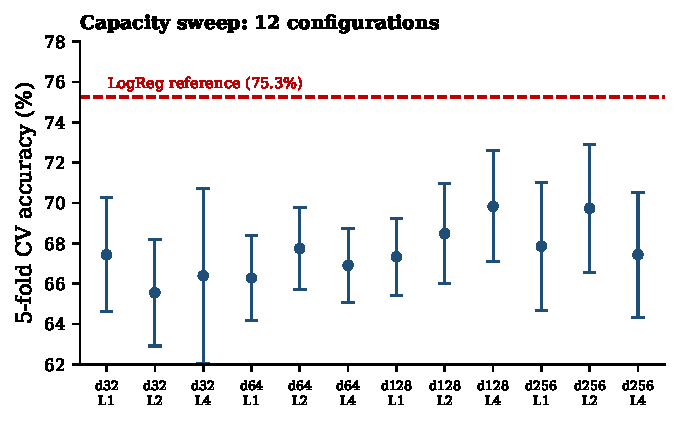
\includegraphics[width=\linewidth]{figures/figB_capacity_sweep.pdf}
\caption{Capacity sweep over 12 configurations ($d \times L$). Every configuration lies below the logistic-regression reference (dashed), and eleven of twelve fall within a 4-point band, indicating that capacity is not the binding constraint.}
\label{fig:capacity_supp}
\end{figure}

\subsection*{S1.2 Learning Curves}

\begin{figure}[htbp]
\centering
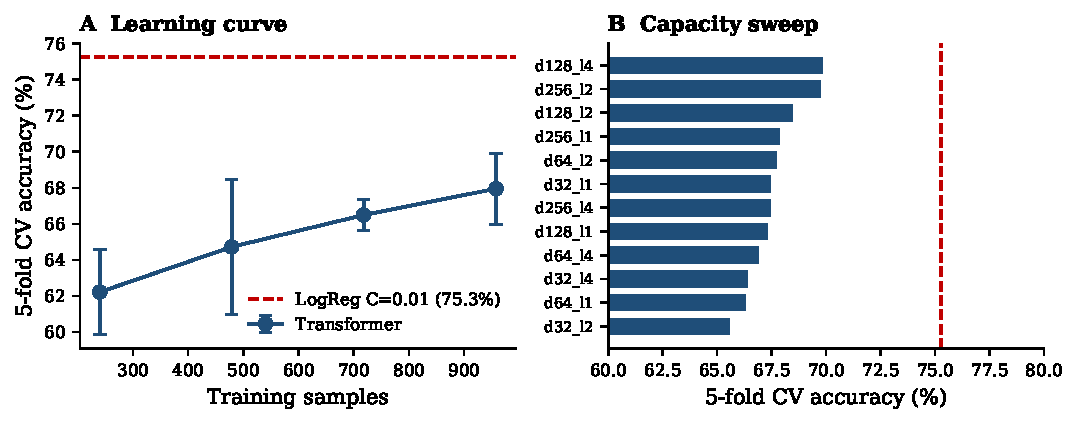
\includegraphics[width=\linewidth]{figures/figA_learning_curves.pdf}
\caption{Learning curve for the best small configuration, with the logistic-regression reference. The curve is decelerating; extrapolation places parity at roughly six times the present training set.}
\label{fig:learning_supp}
\end{figure}

\subsection*{S1.3 Regularization Sweep}

\begin{figure}[htbp]
\centering
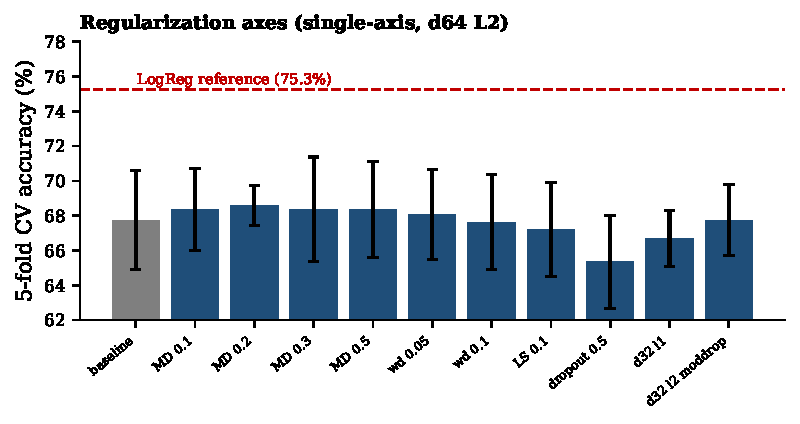
\includegraphics[width=\linewidth]{figures/figC_regularization.pdf}
\caption{Single-axis regularization sweep. The strongest intervention gains 0.84 points, and no configuration approaches the logistic-regression reference.}
\label{fig:regularization_supp}
\end{figure}

\subsection*{S1.4 Pretraining Results}

\begin{figure}[htbp]
\centering
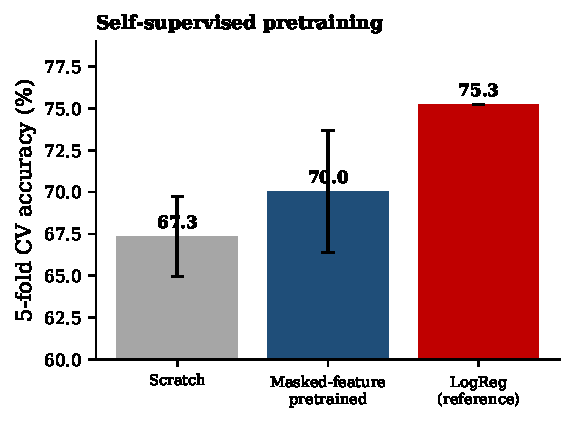
\includegraphics[width=0.7\linewidth]{figures/figD_pretraining.pdf}
\caption{Masked-feature pretraining raises cross-validated accuracy by 2.7 points, the largest internal gain of any intervention tested, without reaching the linear reference.}
\label{fig:pretraining_supp}
\end{figure}

\subsection*{S1.5 External Validation Reversal}

\begin{figure}[htbp]
\centering
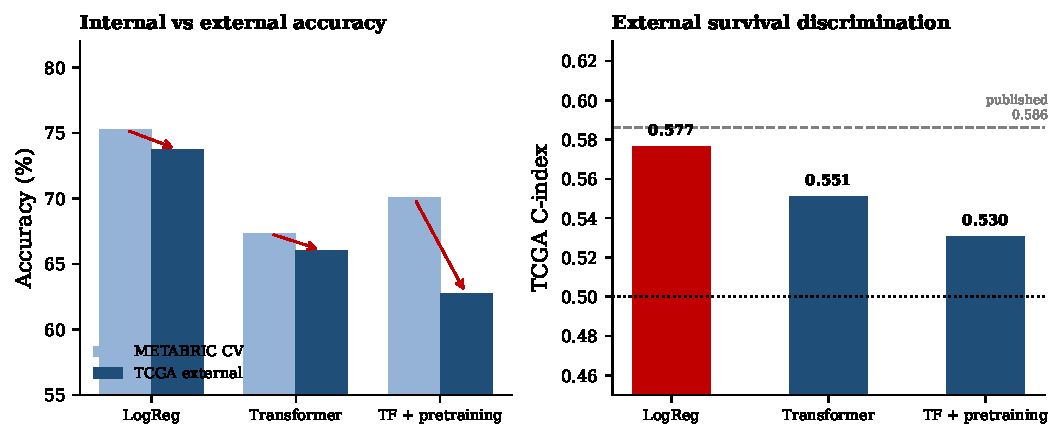
\includegraphics[width=\linewidth]{figures/figE_tcga_validation.pdf}
\caption{Internal versus external performance. Left: accuracy on METABRIC cross-validation and on TCGA. Right: external survival C-index. The pretrained Transformer shows the largest internal-to-external drop, and the lowest external C-index.}
\label{fig:route_a_tcga_supp}
\end{figure}

\subsection*{S1.6 Supplementary Tables}

\begin{table}[htbp]
\centering
\caption{Complete feature engineering details for all five modalities.}
\label{tab:features_supp}
\begin{tabular}{llll}
\toprule
\textbf{Modality} & \textbf{Variables} & \textbf{Encoding} & \textbf{Dimensions} \\
\midrule
Clinical & 22 variables & One-hot + Z-score & 69 \\
mRNA & 412 genes & Z-score & 412 \\
CNA & 256 genes & Z-score & 256 \\
Methylation & 232 probes & Z-score & 232 \\
Mutation & 173 genes & Binary & 173 \\
\midrule
\textbf{Total} & \textbf{1,095} & & \textbf{1,142} \\
\bottomrule
\end{tabular}
\end{table}

\begin{table}[htbp]
\centering
\caption{ANOVA feature selection results for mRNA genes.}
\label{tab:feature_selection_supp}
\begin{tabular}{lcc}
\toprule
\textbf{Gene} & \textbf{F-statistic} & \textbf{Rank} \\
\midrule
ACOT4 & 130.8 & 1 \\
A2ML1 & 102.0 & 2 \\
ABAT & 98.5 & 3 \\
\vdots & \vdots & \vdots \\
\bottomrule
\end{tabular}
\end{table}


\section*{S2. Five-Class Training Baselines}
\label{supp:fiveclass}

The main text trains a six-class METABRIC model and reconciles its output space at
evaluation time. An alternative is to train directly on five classes. We built both
five-class variants from the same 412-gene rank-normalised mRNA features and the same
$C{=}0.01$ logistic regression: \emph{drop} removes the 91 claudin-low training samples
(n=867), and \emph{merge} relabels them as Basal-like (n=958). Both are evaluated on the
same external cohorts as the six-class estimator.

\begin{table}[H]
\centering
\caption{Five-class training baselines against the six-class estimator with label-space
reconciliation. All rows use one rank-normalised mRNA feature set and logistic regression
($C{=}0.01$); rows differ only in training label space and post-hoc handling.
ECE is computed on top-1 confidence with 15 bins; the Brier score is the multiclass
sum-of-squares.}
\label{supp:tab:fiveclass}
\begin{tabular}{llrrrr}
\toprule
\textbf{Cohort} & \textbf{Estimator} & \textbf{Acc (\%)} & \textbf{Macro F1} & \textbf{ECE} & \textbf{Brier} \\
\midrule
    \multicolumn{6}{l}{\textit{TCGA-BRCA} (n=987)} \\
    \quad 6-class base            &       & 73.76 & 0.585 & 0.0352 & 0.3756 \\
    \quad 6-class mask\_only       &       & 79.74 & 0.757 & 0.0557 & 0.2906 \\
    \quad 6-class em\_pam50        &       & \textbf{80.65} & 0.737 & 0.0460 & \textbf{0.2745} \\
    \quad 5-class drop (n=867)     &       & 80.04 & \textbf{0.774} & 0.0560 & 0.2892 \\
    \quad 5-class merge            &       & 76.90 & 0.695 & 0.0344 & 0.3284 \\
    \midrule
    \multicolumn{6}{l}{\textit{GSE21653} (n=266)} \\
    \quad 6-class base            &       & 63.16 & 0.504 & 0.0836 & 0.4920 \\
    \quad 6-class mask\_only       &       & 68.42 & 0.626 & 0.0364 & 0.4271 \\
    \quad 6-class em\_pam50        &       & \textbf{74.06} & 0.683 & 0.0595 & \textbf{0.3776} \\
    \quad 5-class drop (n=867)     &       & 69.55 & \textbf{0.643} & 0.0467 & 0.4025 \\
    \quad 5-class merge            &       & 72.18 & 0.654 & 0.0481 & 0.3747 \\
    \bottomrule
\end{tabular}
\end{table}

Two observations follow directly. First, on TCGA-BRCA the five-class \emph{drop} model
reaches 80.04\% against 80.65\% for the six-class estimator with EM correction, and the
paired McNemar test does not separate them ($p{=}0.504$): for this cohort, training on five
classes is an equally good route to the same accuracy, and it attains the highest macro F1
of any row (0.774). Second, on GSE21653 the six-class estimator with EM correction is
significantly better than the five-class drop model (74.06\% against 69.55\%, $p{=}0.0033$),
because EM additionally re-estimates the target class priors, which the basal-enriched
composition of that cohort warrants. The \emph{merge} variant is worse than both on TCGA
($p{=}8.0e-06$ against the six-class estimator) and statistically indistinguishable from it on
GSE21653 ($p{=}0.23$).

The honest reading is that label-space \emph{reconciliation} accounts for most of the
recovered accuracy on TCGA, and prior correction adds materially only on the harder cohort.
This does not weaken the main claim -- the reported six-class score of 73.76\% is still an
artefact of the evaluation protocol -- but it does mean that a five-class training run is a
legitimate alternative when the target label space is known \emph{a priori}.


\section*{S3. Calibration of the Corrected Estimates}
\label{supp:calibration}

One objection to prior correction is that it may only redistribute probability mass
towards the dominant class without producing better probability estimates. The ECE and
Brier columns of Table~\ref{supp:tab:fiveclass} test that directly, on the same
predictions. The multiclass Brier score improves monotonically along
base $\rightarrow$ mask\_only $\rightarrow$ em\_pam50 on both cohorts
(TCGA: 0.3756 $\rightarrow$ 0.2906 $\rightarrow$ 0.2745; GSE21653: 0.4920 $\rightarrow$ 0.4271
$\rightarrow$ 0.3776). The corrected probabilities are therefore closer to the observed
outcomes in a proper scoring sense; the correction is not a pure relabelling of the
argmax. ECE moves in the opposite direction at the mask step on TCGA (0.0352 $\rightarrow$
0.0557) because restricting the label space sharpens the confidence distribution while the
residual error is concentrated in the remaining classes; this is why we report both
metrics rather than either alone.


\section*{S4. Paired Significance Tests}
\label{supp:significance}

Table~\ref{supp:tab:mcnemar} reports McNemar tests with continuity correction between
successive estimator stages, on the identical target samples.

\begin{table}[H]
\centering
\caption{McNemar tests (continuity-corrected) between estimator stages. $b$ is the number
of samples the first estimator gets right and the second gets wrong; $c$ is the converse.}
\label{supp:tab:mcnemar}
\begin{tabular}{llrrrr}
\toprule
\textbf{Cohort} & \textbf{Comparison} & \textbf{$b$} & \textbf{$c$} & \textbf{$\chi^2$} & \textbf{$p$} \\
\midrule
    TCGA-BRCA & base\_vs\_mask & 0 & 59 & 57.02 & $4.3e-14$ \\
    TCGA-BRCA & mask\_vs\_em & 20 & 29 & 1.31 & 0.2531 \\
    TCGA-BRCA & base\_vs\_em & 13 & 81 & 47.76 & $4.8e-12$ \\
    TCGA-BRCA & sixclass\_em\_vs\_fiveclass\_drop & 31 & 25 & 0.45 & 0.5040 \\
    TCGA-BRCA & sixclass\_em\_vs\_fiveclass\_merge & 51 & 14 & 19.94 & $8.0e-06$ \\
    \midrule
    GSE21653 & base\_vs\_mask & 0 & 14 & 12.07 & $5.1e-04$ \\
    GSE21653 & mask\_vs\_em & 1 & 16 & 11.53 & $6.9e-04$ \\
    GSE21653 & base\_vs\_em & 1 & 30 & 25.29 & $4.9e-07$ \\
    GSE21653 & sixclass\_em\_vs\_fiveclass\_drop & 13 & 1 & 8.64 & 0.0033 \\
    GSE21653 & sixclass\_em\_vs\_fiveclass\_merge & 8 & 3 & 1.45 & 0.2278 \\
    \bottomrule
\end{tabular}
\end{table}

Two conclusions hold on both cohorts. The label-space step is unambiguous: it fixes 59
samples on TCGA and 14 on GSE21653 while breaking none, and both tests are decisive
($p{=}4.3\times10^{-14}$ and $p{=}5.1\times10^{-4}$). The subsequent EM prior correction is
significant on GSE21653 ($p{=}6.9\times10^{-4}$) but not on TCGA ($p{=}0.25$), consistent
with the accuracy table: prior correction pays off where the target composition departs
substantially from the source.


\section*{S5. Generalising the Absence Pattern Beyond Claudin-Low}
\label{supp:absence}

The analysis in the main text is built on one absent class, claudin-low, in two
PAM50-annotated cohorts. A fair objection is that claudin-low happens to be the rarest
class in the source prior, so the reported effect may be the smallest instance of a
larger phenomenon rather than a representative one. This section removes that
ambiguity by sweeping absence over two axes: \emph{who} is absent, and \emph{how} they
are absent. The protocol is otherwise the one described in the Methods: the same
$C{=}0.01$ logistic regression on the 412-gene rank-normalised mRNA panel, a synthetic
target of $n{=}1000$ drawn from the pooled held-out METABRIC validation and test
splits, and 10 seeds per cell. METABRIC source priors are
LumA %.3f, LumB %.3f, Her2 %.3f, Basal %.3f, claudin-low %.3f, Normal %.3f.

\subsection*{S5.1 Who is absent: severity tracks prior mass, not identity}

\begin{table}[H]
\centering
\caption{Single-class absence, complete (\emph{drop}, target prevalence exactly zero)
and partial (\emph{rare}, target prevalence scaled to $10\%$ of source). Rows are ordered
by descending source prevalence. Bold marks the two commonest classes. Detection F1 is
the label-free procedure's agreement with the true absent set.}
\label{supp:tab:who}
\begin{tabular}{lrrrrrr}
\toprule
& & \multicolumn{2}{c}{\textbf{drop}} & & \multicolumn{2}{c}{\textbf{rare}} \\
\cmidrule(lr){3-4}\cmidrule(lr){6-7}
\textbf{Absent class} & \textbf{Source prior} & \textbf{Naive} & \textbf{Corrected} & \textbf{Gain} & \textbf{Corrected} & \textbf{Det.\ F1} \\
\midrule
    \textbf{LumA} & 0.357 & 74.67 & 86.00 & $+11.33$ & 75.97 & 0.000 \\
    \textbf{LumB} & 0.239 & 78.10 & 88.51 & $+10.41$ & 85.93 & 0.067 \\
    Her2 & 0.125 & 78.82 & 81.51 & $+2.69$ & 82.53 & 0.900 \\
    Basal & 0.104 & 79.25 & 80.30 & $+1.05$ & 79.89 & 0.900 \\
    CL & 0.095 & 79.17 & 80.91 & $+1.74$ & 79.85 & 0.967 \\
    Normal & 0.079 & 79.34 & 81.51 & $+2.17$ & 81.08 & 0.800 \\
    \bottomrule
\end{tabular}
\end{table}

The result is unambiguous. Removing \textbf{Luminal A}, the commonest class, costs
11.33 points of naive accuracy and all of it is recoverable ($74.67\% \rightarrow
86.00\%$). Removing claudin-low costs 1.74 points. The severity of a label-space
mismatch is therefore governed by the \emph{prior mass} of the absent class, not by its
identity: claudin-low is the mildest instance of the phenomenon, not a representative
one, and a cohort that omits a common subtype would show an effect an order of magnitude
larger.

The partial-absence column (\emph{rare}) exposes a second, less comfortable result. When
the class is under-ascertained rather than absent outright, the label-free detector
essentially fails for the common classes: detection F1 is
\textbf{0.000} for Luminal A and \textbf{0.067} for Luminal B, against 0.967 for
claudin-low. A class that is merely heavily under-counted leaves a probability marginal
indistinguishable from a genuinely rare class, which is precisely the identifiability
failure the main text reports, now shown to be worst exactly where the stakes are
highest.


\subsection*{S5.2 How it is absent: merging is worse than dropping}

Real annotation disagreement rarely takes the form of a class vanishing. More often a
cohort folds one class into a neighbour's label -- claudin-low recorded as Basal-like,
or Luminal B recorded as Luminal A. We simulate this by moving the absent class's prior
mass onto the neighbour instead of discarding it.

\begin{table}[H]
\centering
\caption{Merge-mode absence: the source class is relabelled as its neighbour.
Naive accuracy is barely affected, because the merge is partly \emph{correct} under the
target's coarser standard; the recoverable loss is correspondingly larger than for a
clean drop.}
\label{supp:tab:how}
\begin{tabular}{llrrrr}
\toprule
\textbf{Pattern} & \textbf{Absent class} & \textbf{Source prior} & \textbf{Naive} & \textbf{Corrected} & \textbf{Gain} \\
\midrule
    LumA$\rightarrow$LumB & LumA & 0.357 & 76.73 & 89.82 & $+13.09$ \\
    LumB$\rightarrow$LumA & LumB & 0.239 & 79.43 & 91.48 & $+12.05$ \\
    Her2$\rightarrow$LumB & Her2 & 0.125 & 79.04 & 81.18 & $+2.14$ \\
    CL$\rightarrow$Basal & CL & 0.095 & 78.39 & 80.38 & $+1.99$ \\
    Normal$\rightarrow$LumA & Normal & 0.079 & 79.36 & 82.04 & $+2.68$ \\
    \bottomrule
\end{tabular}
\end{table}

Luminal B merged into Luminal A -- the exact pattern a reader is most likely to meet in
practice -- leaves naive accuracy at 79.43\% while hiding a recoverable loss of 12.0
points. This is the most consequential cell in the whole simulation, and it involves
neither a rare class nor a class vanishing: two subtypes with the same receptor status
and overlapping expression, recorded under one label. Detection F1 here is 0.767, so the
label-free procedure does not rescue it.

\subsection*{S5.3 Multiple absences}

Dropping every pair of classes (15 combinations) gives a recoverable loss between
$+1.41$ and $+17.31$ points, and the ordering again follows the combined prior mass:
the worst cell is Luminal A with Luminal B ($+17.31$ points, naive accuracy 66.01\%),
the mildest is claudin-low with Basal-like ($+1.41$). Detection F1 is high across most
pairs (1.000 in 11 of 15 cells) because two simultaneously suppressed classes produce a
stronger simplex signal than one; the failures are concentrated in the pairs whose
members are individually hardest to separate (claudin-low with Basal-like, 0.860).

Taken together, Supplementary Tables~\ref{supp:tab:who} and~\ref{supp:tab:how} support
the main text's recommendation and sharpen it. The rule "establish the target's allowed
labels from cohort documentation" is not a precaution against an exotic failure mode. It
is the only reliable remedy for a mismatch whose magnitude ranges over two orders of
magnitude depending on which class the annotation standard omits, and whose most likely
real-world form -- a class merged into its neighbour -- is the one that hides the most.

\end{document}
